\subsection{Enunciado}
Dos hermanos fueron separados al nacer y mediante un programa de televisión se han
enterado que podrían ser hermanos. Ante esto, los dos están de acuerdo en hacerse un test de
ADN para verificar si realmente son hermanos. Se debe encontrar el porcentaje de similitud que existe 
entre estos posibles hermanos, $($como es un ejemplo lo haremos para 2 entradas posibles$)$.

\subsection{Metodología} \label{sec:metodologia}

\begin{figure}[h]
  \centering
  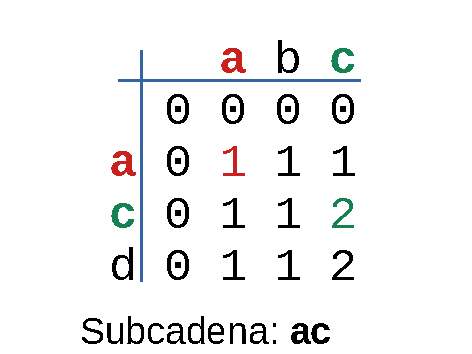
\includegraphics[scale=0.6]{img/dibujito.pdf}
  \caption{Ilustración del funcionamiento del algoritmo basado en programación dinámica.}
\end{figure}

Para llevar a cabo este algoritmo mediante programación dinámica vamos a construir la matriz de 
ocurrencias. Para ello vamos a construir una función que la calcule y luego la implementaremos.

Sean $n,m \in \mathbb{N}$, dadas dos secuencias $X = { x_1,x_2,...,x_m}$ e $Y = { y_1,y_2,...,y_n}$, llamaremos $L(i,j)$ a la 
longitud de la secuencia común máxima de las secuencias $X_i = {x_1,...,x_i}$ e $Y_j = {y_1,...,y_j}$ $\forall i \in {1,...,n} $ y $\forall i \in {1,...,m}$, 
que se define como:  

\[
  L(i,j) = 
  \left \{
    \begin{aligned}
      0 &,\ \text{si} \ i = 0 \ o \ j = 0\\
      L(i,j) + 1 &,\ \text{si} \ i \neq  1 , j \neq  0 \ y \ x_i = y_j\\
      max(L(i,j-1) , L(i-1,j))&,\ \text{si} \ i \neq 1 , j \neq 0 \ y \ x_i \neq y_j
    \end{aligned}
  \right .
\]

En esta matriz tenemos que hacer que cada elemento de la cadena X sea una posición de cada columna 
y cada elemento de la cadena Y ocupe una posición de cada fila. Con esta disposición, vamos recorriendo
la matriz por filas y si fijado el elemento de cada fila encontramos un elemento igual que esté en una 
posición de las columnas, incrementamos la longitud, en caso contrario, cogemos el máximo entre el valor de 
la fila y la columna correspondiente.

\subsubsection{Pseudocódigo}

\begin{algorithm}[H]
  \caption{Algoritmo para la matriz que calcula la subsecuencia con mayor similitud.}\label{alg:simil}
  \begin{minipage}{0.92\textwidth}
  \textbf{Parámetro}: string (palabra1)
  \textbf{Parámetro}: string (palabra2)
  \textbf{Parámetro}: string (subsecuencia)
  \textbf{Parámetro}: int (longitud=0)
  \end{minipage}

  int matriz[MAX][MAX] = {0}

  \For{i desde 1 $\leq$ palabra1.size y ++i} {
    \For{j desde 1 $\leq$ palabra2.size y ++j} {
      \eIf{palabra1[i-1] == palabra2[j-1]}{
        matriz[i][j] = matriz[i-1][j-1]+1\;
      }{ matriz[i][j] = max(matriz[i][j-1],matriz[i-1][j])\;}
    }
  }
\end{algorithm}

\subsubsection{Implementación}
\lstinputlisting[label={cod:simil}, firstline=26, lastline=36, language=C++,
caption=Algoritmo para la matriz que calcula la subsecuencia con mayor similitud.]{../src/similitud.cpp}

\subsection{Aplicabilidad de la programación dinámica}

Como se ha discutido previamente, para aplicar un algoritmo basado en programación
dinámica se ha de verificar las siguientes condiciones:

\begin{enumerate}
    \item Comprobación de la naturaleza n-etápica del problema. 
    \item Verificación del principio de optimalidad de Bellman. 
    \item Construcción de una ecuación recurrente. 
    \item Cálculo de la solución(enfoque adelantado o retardado). 
\end{enumerate}

\subsubsection{Naturaleza n-etápica}
En efecto, 
% para encontrar la subsecuencia $c_n$ más larga de longitud n, hemos de empezar 
% previamente con las subsecuencias más largas de longitud 1,2... ($c_1$, $c_2$, ...). 
como primera etapa se ha de conseguir las subsecuencias más largas de longitud 1, 
después obtener las subsecuencias más largas de longitud 2 y, así, sucesivamente. 


\subsubsection{Verificación del principio de optimalidad de Bellman}

En esta parte, vamos a determinar que el problema que hemos expuesto verifica,
efectivamente, el principio de optimalidad de Bellman. Para ello, veamos que el
problema verifica una subestructura optimal. El método y el teorema se pueden encontrar
en \cite{Cormen2017}. 

\textbf{Notación}. Sea $X$ una secuencia de caracteres. Definimos \textbf{prefijo i-ésimo}
de X, notado por $X_i$, al vector formado por los i primeros elementos de $X$. 
También definimos por \textbf{subsecuencia común} a dos secuencias de caracteres $X,Y$ a cualquier sucesión de caracteres
cuyo orden ascendente se encuentre tanto en $X$ como en $Y$. Además, diremos que la
subsecuencia común es \textbf{máxima} cuando su número de caracteres sea igual o superior 
a cualquier otra subsecuencia común. 

\begin{theorem}
    Sean $X=(x_1,x_2,\cdots, x_m),Y=(y_1,y_2, \cdots, y_n)$ secuencias de caracteres 
    y sea $Z$ cualquier subsecuencia común máxima 
    de $X$ e $Y$. Entonces:
    \begin{enumerate}
      \item Si $x_m = y_n$, entonces $z_k = x_m = y_n$ y $Z_{k-1}$ es una subsecuencia
      común máxima de $X_{m-1}$ e $Y_{n-1}$. 
      \item Si $x_m \neq y_n$, entonces:
      \begin{enumerate}
        \item $z_k \neq x_m$ implica que $Z$ es una subsecuencia común máxima para $X_{m-1}$ e $Y$. 
        \item $z_k \neq y_n$ implica que $Z$ es una subsecuencia común máxima para $X$ e $Y_{n-1}$. 
      \end{enumerate}
    \end{enumerate}
\end{theorem}
% Pag 392

\begin{proof}
  Empezamos probando (1). Supongamos que $x_m = y_n$. Si fuese $z_k \neq x_m$,
  podríamos añadir $x_m = y_n$ para obtener una subsecuencia común de $X$ e $Y$ 
  de longitud k+1, contradiciendo la hipótesis de subsecuencia común máxima de Z. 
  Por tanto, ha de ser $z_k = x_m = y_n$. Ahora, el prefijo $Z_{k-1}$ es una
  subsecuencia común de k-1 caracteres, subsecuencia común de $X_{m-1}$ e $Y_{n-1}$.
  Veamos que se trata de una subsecuencia común máxima. Para ello, procedemos
  nuevamente por reducción al absurdo. Supongamos que existe una subsecuencia común $W$ de
  $X_{m-1}$ e $Y_{n-1}$ con longitud mayor que $k-1$. Entonces, añadiendo $x_m$ a $W$
  se produce una subsecuencia común de $X$ e $Y$ cuya longitud es mayor que k, lo
  que sería contradictorio.

  Para (2), empezamos probando el primero. Si $z_k \neq x_m$, entonces $Z$ es una
  subsecuencia común de $X_{m-1}$ e $Y$. Si hubiese una subsecuencia común $W$
  de longitud mayor que $k$, entonces $W$ sería nuevamente una subsecuencia común 
  de $X_m$ e $Y$, contradiciendo que $Z$ sea una subsecuencia común máxima.
  Análogamente se haría para el caso $z_k \neq y_n$. 
\end{proof}

Este teorema demuestra que el problema verifica el principio de optimalidad de
Bellman, pues cualquier política óptima únicamente puede estar formado por
subpolíticas óptimas. 

\subsubsection{Construcción de la ecuación recurrente}

Construimos ahora la ecuación recurrente asociada. Ello lo haremos aplicando
la expresión de $C_{ij}$ que aparece en la Sección~\ref{sec:metodologia}, por lo
que, efectivamente, se trata de una expresión recurrente. 

\subsubsection{Cálculo de la solución}

Para resolver el problema hemos propuesto el pseudocódigo que vamos a presentar
a continuación. 

\subsection{Pseudocódigo}

\subsection{Implementación}

La implementación del algoritmo del algoritmo de similitud en C++ usando la técnica programación dinámica es la siguiente:


\lstinputlisting[label={cod:cod-pd}, firstline=20, lastline=63, language=C++,
caption=Implementación del algoritmo de similitud basado en PD.]{../src/similitud.cpp}


\subsection{Análisis de eficiencia teórico}

A continuación, analizaremos la eficiencia del algoritmo en notación asintótica $BigO$.
Llamamos $n$ a la longitud de las secuencias (ambas tienen el mismo número de componentes). En primer lugar nos encontramos con un doble ciclo for que recorre ambas
secuencias y contiene operaciones $O(1)$, luego la eficiencia del bloque es $O(n^{2})$.
Posteriormente tenemos sentencias de asignación que serán despreciadas, y llegamos a un
ciclo while que realiza $n$ iteraciones, en cuyo interior tenemos operaciones elementales que son $O(1)$, y finalmente obtemos la subsecuencia con otro bucle while, que puede realizar un número inferior o igual a $n$ operaciones. Por tanto, aplicando la regla del máximo, obtenemos que \textbf{nuestro algoritmo tiene una eficiencia de $O(n^{2})$}.
 

\subsection{Resultados}

Ahora vamos a resolver el programa planteado inicialmente. Para ello,
hemos ejecutado los códigos tanto para el primer como para el segundo caso,
obteniendo las Tablas \ref{tab:s1} y \ref{tab:s2}. También podemos encontrar
una captura de la salida del programa para el primer caso en la Figura~\ref{fig:1}. 

\begin{table}[h]
    \footnotesize
    \centering
	\begin{tabular}{|l|l|l|ll}
		\cline{1-3}
		\textbf{Secuencias}                           & \textbf{Subsecuencia común máxima}                       & \textbf{Porcentaje de similitud}     &  &  \\ \cline{1-3}
		abbcdefabcdxzyccd                    & \multirow{2}{*}{abbcdefbcdxyccd}                & \multirow{2}{*}{$88 \%$}    &  &  \\ \cline{1-1}
		abbcdeafbcdzxyccd                    &                                                 &                             &  &  \\ \cline{1-3}
	\end{tabular}
  \caption{Datos obtenidos de la comparación de las secuencias de caracteres.}
  \label{tab:s1}
\end{table}

\begin{table}[h]
  \footnotesize
  \centering
\begin{tabular}{|l|l|l|ll}
  \cline{1-3}
  \textbf{Secuencias}                           & \textbf{Subsecuencia común máxima}                       & \textbf{Porcentaje de similitud}     &  &  \\ \cline{1-3}
  010111000100010101010010001001001001 & \multirow{2}{*}{100001000101010001000100100100} & \multirow{2}{*}{$83.33 \%$} &  &  \\ \cline{1-1}
  110000100100101010001010010011010100 &                                                 &                             &  &  \\ \cline{1-3}
\end{tabular}
\caption{Datos obtenidos de la comparación de las secuencias de números.}
\label{tab:s2}
\end{table}

\begin{figure}
  \centering
  \caption{Salida para el primer caso.}
  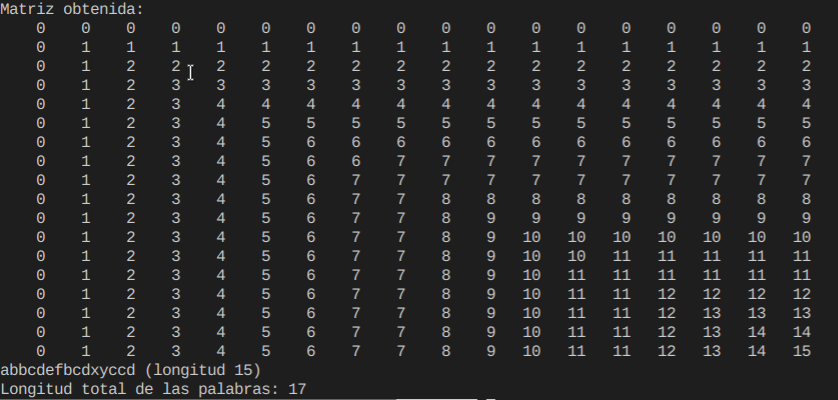
\includegraphics[scale=0.67]{img/LettersMatrixResult.png}
  \label{fig:1}
\end{figure}

\subsection{Comparación con el algoritmo de fuerza bruta}

En este apartado vamos a presentar una resolución alternativa del problema
usando un algoritmo de fuerza bruta, y compararemos sus prestaciones con el
algoritmo que emplea programación dinámica anteriormente tratado.

En cuanto a su funcionamiento, se trata de formar dos conjuntos, uno para cada cadena, que contengan todos los subconjuntos que pueden formarse considerando los elementos de la cadena, respetando el orden relativo de los elementos (un elemento se encuentra a la izquierda o a la derecha del otro), pero no el orden absoluto (los elementos no deben de ser adyacentes). Una vez obtenemos estos dos conjuntos, comparamos los subconjuntos de las dos cadenas y nos quedamos con el subconjunto 
o subcadena común de mayor longitud.

Su implementación en C++ sería la siguiente:

\lstinputlisting[label={cod:cod-fb}, firstline=13, lastline=90, language=C++,
caption=Implementación del algoritmo de similitud basado en fuerza bruta.]{../src/fbruta.cpp}

En cuanto al análisis de eficiencia teórico de este algoritmo, como tenemos que calcular el conjunto de las partes de un conjunto, operación realizada en la función 
\texttt{subcadenasPalabra} que es de un orden de complejidad de $O(2^{n})$, aplicando la regla del máximo con el resto de funciones que tienen complejidad polinómica, obetenmos que \textbf{la eficiencia del algoritmo es de $O(2^{n})$}.

En comparación con el algoritmo basado en programación dinámica, \textbf{el orden de eficiencia del algoritmo de fuerza bruta es no polinomial, superior al que proporciona la PD}, esto hace que su tiempo de ejecución sea mayor, de forma que podemos apreciar una notable diferencia en cuanto a los tiempos a partir de un 
tamaño de $n=10$, luego no tiene sentido realizar ejecuciones con este algoritmo
para valores mayores, usaremos en su lugar el algoritmo basado en PD.

